\documentclass[xelatex,ja=standard,a4paper,14pt,everyparhook=compat]{bxjsarticle}
\usepackage{amsmath, amssymb, amsthm}
\usepackage{mathtools, bm}
\usepackage{enumerate}

% \usepackage{concmath}
% \usepackage[OT1]{fontenc}
% \setsansfont{CMU Concrete}
% \setmainfont{CMU Concrete}
% \setCJKmainfont{Noto Sans JP Light}
% \setCJKsansfont{Noto Sans JP Light}

\newcommand{\paren}[1]{\left(#1\right)}

\newcommand{\bbC}{\mathbb{C}}
\newcommand{\bbN}{\mathbb{N}}
\newcommand{\bbP}{\mathbb{P}}
\newcommand{\bbF}{\mathbb{F}}
\newcommand{\frakS}{\mathfrak{S}}
\DeclareMathOperator{\inv}{inv}

\theoremstyle{definition}
\newtheorem{theorem}{定理}[subsection]
\newtheorem*{theorem*}{定理}
\newtheorem{example}[theorem]{例}
\newtheorem*{example*}{例}
\newtheorem{definition}[theorem]{定義}
\newtheorem*{definition*}{定義}
\newtheorem{proposition}[theorem]{命題}
\newtheorem{corollary}[theorem]{系}
\renewcommand{\proofname}{\textup{証明}}

\begin{document}

\setcounter{section}{2}
\section{Partially Ordered Sets}
\subsection{Basic Concepts}

この章で扱われる半順序集合(partially ordered set, poset)は数え上げで統一的な役割を果たす.

主なトピック:\begin{itemize}
    \item メビウス反転(包除原理の一般化など)
    \item Binomial posets(さまざまな母関数の統一)
\end{itemize}

\begin{example*}
    有限集合$A,B,C,D$について \begin{equation*}
        D = A \cap B = A \cap C = B \cap C = A \cap B \cap C
    \end{equation*}
    であるような状況を考える.包除原理より \begin{align*}
        |A \cup B \cup C|
         & = |A| + |B| + |C| - |A \cap B| - |A \cap C| - |B \cap C| \\
         & \phantom{={}} + |A \cap B \cap C|                        \\
         & = |A| + |B| + |C| - 2|D|.
    \end{align*}
    この$-2$はどこから来たのか?より一般に,$A_1,\ldots,A_n$の交差に対してこれらの係数を効率的に計算できるか?
\end{example*}

\begin{definition*}
    \textbf{半順序集合}$P$ (\textbf{partially ordered set}, \textbf{poset})は,集合$P$と次の公理を満たす二項関係$\leq$ (より明確には$\leq_P$)からなる. \begin{enumerate}
        \item 任意の$t \in P$について$t \leq t$ (反射律)
        \item $s \leq t$,$t \leq s$ならば$s = t$ (反対称律)
        \item $s \leq t$,$t \leq u$ならば$s \leq u$ (推移律)
    \end{enumerate}
    $t \geq s$は$s \leq t$の意味.また,$s < t$は``$s \leq t$かつ$s \neq t$'',$t > s$は$s < t$の意味.

    $s \leq t$または$t \leq s$が成り立つとき$s,t \in P$は\textbf{比較可能}(\textbf{comparable}).そうでないときは\textbf{比較不可能}(\textbf{incomparable})といい,$s \parallel t$で表す.
\end{definition*}

\begin{example}
    Posetの例

    \begin{enumerate}[a.]
        \item $\pmb{n}$:$n > 0$について,集合$[n]$を通常の順序で順序付けたもの.
        \item $B_n$:$n \geq 0$について,$[n]$の部分集合全体を包含関係で順序付けたもの.
        \item $D_n$:$n > 0$について,$n$の約数全体を \begin{equation*}
                  i \leq j \ \overset{\mathrm{def}}{\Longleftrightarrow} \ \text{$i$は$j$を割り切る}
              \end{equation*}
              で順序付けたもの.
        \item $\Pi_n$:$n > 0$について,$[n]$の分割\footnote{有限集合$X$と$B_1,\ldots,B_k \subseteq X$について以下の条件が成り立つとき,$\{B_1, \ldots, B_k\}$は$X$の\textbf{分割}であるという. \begin{enumerate}
                      \item $B_i \neq \emptyset$,
                      \item $\bigcup_i B_i = X$,
                      \item $i \neq j$ならば$B_i \cap B_j = \emptyset$.
                  \end{enumerate}}全体を \begin{equation*}
                  \pi \leq \sigma \ \overset{\mathrm{def}}{\Longleftrightarrow} \ \text{$\pi$は$\sigma$の細分}\footnote{$\pi$のどのブロックもある$\sigma$のブロックの部分集合であるとき,$\pi$は$\sigma$の細分であるという.}
              \end{equation*}
              で順序付けたもの.
        \item $B_n(q)$:$n$次元ベクトル空間$\bbF_q^n$の部分空間全体を包含関係によって順序付けたもの.
    \end{enumerate}
\end{example}

\newpage

\begin{definition*}
    Poset $P, Q$について, \begin{equation*}
        s \leq t \ \Longleftrightarrow \ \phi(s) \leq \phi(t)
    \end{equation*}
    なる全単射$\phi \colon P \to Q$が存在するとき,$P$と$Q$は\textbf{同型(isomorphic)},$P \cong Q$.
\end{definition*}

\begin{definition*}
    Poset $P,Q$について,$Q \subseteq P$かつ \begin{equation*}
        s \leq_Q t \ \Longrightarrow \ s \leq_P t
    \end{equation*}
    であるとき,$Q$は$P$の\textbf{弱部分半順序集合(weak subposet)}.さらに集合として$P=Q$であるとき,$P$は$Q$の\textbf{細分(refinement)}.

    また,$Q \subseteq P$について \begin{equation*}
        s \leq_Q t \ \Longleftrightarrow \ s \leq_P t \qquad (s,t \in Q)
    \end{equation*}
    が成り立つとき,$Q$は$P$の\textbf{誘導部分半順序集合(induced subposet)},または単にsubposet.

    $s \leq t$に対して,\textbf{(閉)区間(interval)}は \begin{equation*}
        [s,t] = \{u \in P : s \leq u \leq t\},
    \end{equation*}
    \textbf{開区間}は \begin{equation*}
        (s,t) = \{u \in P : s < u < t\}.
    \end{equation*}

    $P$のすべての区間が有限集合であるとき,$P$は\textbf{局所有限(locally finite)}.$P$のsubposet $Q$について \begin{equation*}
        s,u \in Q, \ s < t < u \ \Longrightarrow \ t \in Q
    \end{equation*}
    が成り立つとき,$Q$は\textbf{凸(convex)}.
\end{definition*}

\newpage

\begin{definition*}
    $s,t \in P$について, \begin{enumerate}
        \item $s < t$,かつ
        \item $s < u < t$なる$u \in P$が存在しない
    \end{enumerate}
    とき,$t$は$s$を\textbf{被覆(cover)}する.$s \lessdot t$,$t \gtrdot s$と表す.

    有限poset $P$について,$P$の元が頂点,被覆関係が辺で表され,$s \lessdot t$であるとき$t$が$s$より上の位置に描かれるようなグラフを\textbf{ハッセ図(Hasse diagram)}という.

    \begin{figure}[h]
        \centering
        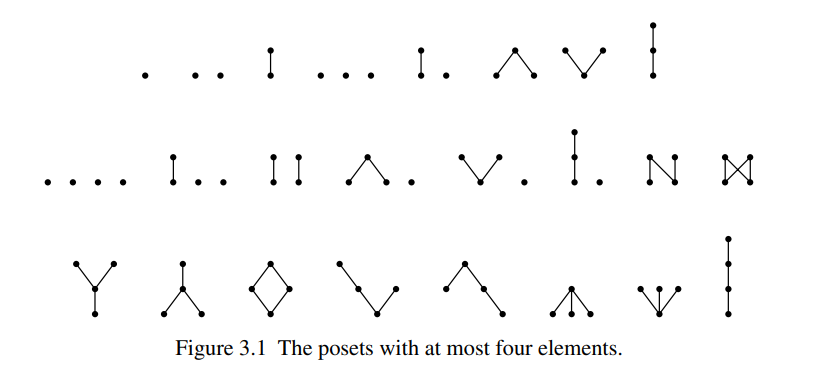
\includegraphics[width=.9\textwidth]{Fig3.1.png}
        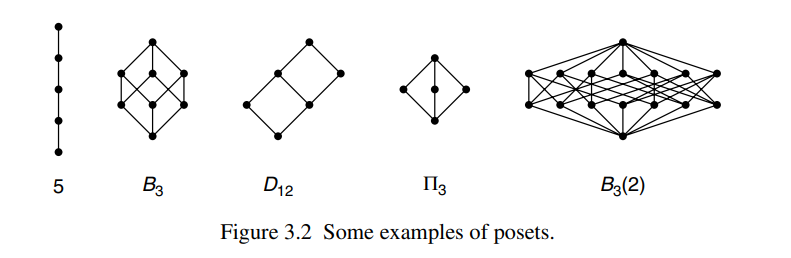
\includegraphics[width=.9\textwidth]{Fig3.2.png}
    \end{figure}
\end{definition*}

\begin{definition*}
    $\forall t \in P$, $t \geq \hat 0$なる$\hat 0$が存在するとき,\textbf{$P$は$\hat 0$を持つ}.

    $\forall t \in P$, $t \leq \hat 1$なる$\hat 1$が存在するとき,\textbf{$P$は$\hat 1$を持つ}.

    $P$に新たに$\hat 0$,$\hat 1$を付け加えたものを$\widehat P$で表す.
\end{definition*}

\section*{演習問題から}

\begin{enumerate}
    \item[2.] \begin{enumerate}[a.]
              \item 集合$P$上の二項関係$\leq$が反射率と推移律を満たすとき,$P$は\textbf{preposet} (\textbf{前順序集合},\textbf{擬順序集合},\textbf{quasi-ordered set})をなす.Preposet $P$と$s,t \in P$について \begin{equation*}
                        s \sim t \ \overset{\mathrm{def}}{\Longleftrightarrow} \ s \leq t \text{かつ} t \leq s
                    \end{equation*}
                    とするとき,$\sim$が同値関係であることを示せ.
              \item $\sim$による$P$の同値類の集合を$\widetilde P$と表す.$S, T \in \widetilde P$について \begin{equation*}
                  S \leq T \ \overset{\mathrm{def}}{\Longleftrightarrow} \ \text{$s \leq t$なる$s \in S$,$t \in T$が存在する}
              \end{equation*}
              とするとき,$\widetilde P$がposetをなすことを示せ.
              \item $Q$をposetとし,写像$f \colon P \to Q$がorder-preservingであるとする.$P$から$\widetilde P$への自然な写像を$\phi$とするとき, \begin{equation*}
                  f = g \circ \phi
              \end{equation*}
              なるorder-preservingな写像$g \colon \widetilde P \to Q$が一意に存在することを示せ.
          \end{enumerate}
    \item[4.] $P$をposetとする.次の条件を満たす集合族$\mathcal{S}$が存在することを示せ. \begin{itemize}
              \item $\mathcal{S}$に半順序 \begin{equation*}
                        S \leq T \ \overset{\mathrm{def}}{\Longleftrightarrow} \ S \subseteq T
                    \end{equation*}
                    を定めると,$\mathcal{S} \cong P$.
          \end{itemize}
    \item[5.] \begin{enumerate}
              \item[b.] 同型でない$n$-元のposetの個数を$f(n)$とする.この$f(n)$の値を与える適当な式は見つかっていない.
              \item[c.] この$f(n)$の値のうち,$10$進法で表記したときに回文となるようなものの個数が無限個あるかは,ZFで証明することも反証することもできない.
          \end{enumerate}
    \item[6.] \begin{enumerate}[a.]
        \item $P$を有限posetとし,$f \colon P \to P$をorder-preservingな全単射とする.$f$が自己同型写像,すなわち$f^{-1}$がorder-preservingであることを示せ.
        \item $P$が有限集合のとき,(a)が一般には成り立たないことを示せ.
    \end{enumerate}
\end{enumerate}

\end{document}
